%cosmics.tex- Technote for UBooNE Cosmogenic background study
\documentclass[10pt]{article}
\usepackage{color}
\usepackage{amsmath}
\usepackage{hyperref}
\usepackage{graphicx}
\usepackage{setspace}
%\singlespace
%\onehalfspacing
%\doublespace
%\linespread{2}

%End preamble, begin document
\begin{document}
\title{ Cosmogenic Background Reduction }
\author{ Authors \\Associated Universities \\
\\MicroBooNE\\ }
\date{\today}
\maketitle

\renewcommand{\abstractname}{Abstract}
\begin{abstract}
A well characterized background is crucial to the successful selection of signal events from data.  In particular, Compton scattered electrons from cosmics may resemble $\nu_e$ electrons, an interaction of primary interest to MicroBooNE.  In this study, we investigate the properties of Compton scatters that mimic a single electron shower signal and attempt to reduce them. 

\end{abstract}

%Set Table of contents depth to 3 levels
\tableofcontents
\setcounter{tocdepth}{1} 
\phantomsection
\clearpage

\section{Introduction}
MicroBooNE, a surface dweller, is subject to constant bombardment of cosmic radiation from the upper atmosphere. Gammas from these upper atmosphere cascades can Compton scatter or pair produce in the detector, resulting in either an electron shower from the former, or electron/positron showers from the latter. These backgrounds have the potential to mimic MicroBooNE's primary signal, a single electron shower (with vertex activity).  To filter these background events from data, we can look at various parameters that may distinguish them from our desired signal. For instance, most gamma radiation comes from above the detector; it is thus reasonable to expect many of the Compton scattered (and pair produced) showers to have a downward trajectory. In addition, the interaction length in Liquid Argon (14cm) limits the distance we can expect a Compton gamma to travel before interacting (DOCDB 3693).   We explore these and other parameters in further detail in this study.

\section{Sample}
There were 2 sets of files used for these tests.  The first are MCC5 generated BNB files with 20,000 events, 121 single electron $\nu_e$ events. The second are cosmic background files generated by Kazu (maybe? ) . More things.  ?


\section{Methodology}
Two separate studies are performed.  
\\ \\In the first, MCC5 generated BNB files are used with (Kazu's) PDG filter to select single electron events.  Information such as energy, vertex activity, vertex coordinates and distances along electron trajectory to detector edge (both forward and backward) are stored for 121 electron events / 20,000 total BNB events.  This is intended to act as a baseline for the second study.  
\\ \\  In the second, the cosmogenic sample described above is examined.  In such a case, there are 2 subsets of interactions to sift through which might mimic our primary signal: Compton scatters and pair production.  A fiducial volume cut guarantees the vertex is inside the detector volume and dE/dx information from the first 2.4cm of a shower can help distinguish gamma from electron activity; we are then able to distinguish between these two interactions in a true sample.  Our first mode of action beyond this is thus to introduce a tag which stores properties of each interaction mode separately (I'm pretty sure I'm going into unnecessary detail here?). Using the selected sample of Compton scatters from Cosmic data, we then investigate properties of the interactions.  In particular, we (will) use geometric algorithms to calculate the distance back along the trajectory from vertex to detector edge.  Combing this information with interaction length, energy and angle, we are able to successfully ( hopefully--not done yet) reduce background Compton scatters while minimally reducing events in the true single electron sample. 


\section{Results}

(Brief discussion of thus far included plots only)

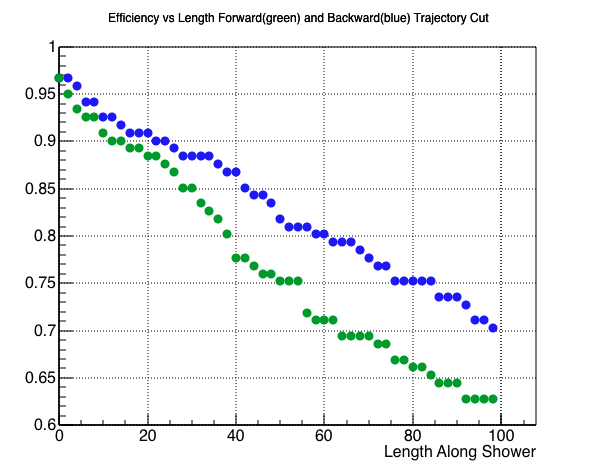
\includegraphics[scale=0.5]{Eff.png}

In the above plot, efficiency is defined as number of events that pass a cut divided by total number of events.This plot is made for the sample of 121 selected single electron events from BNB files described above.  The blue dots show the efficiency of this sample for length cuts backwards along the trajectory to the detector wall.  Comparing this to cosmogenic data (haven't done this yet), we see that for X cm length cut, Y \% of electron events remain. 
	
\section{Llamas}
\subsection{Llamas 1.0: Llama Environment}
\subsection{Llamas 2.0: Llama Hygiene}
\subsection{Llamas 3.0: What Gives the Llama its Jive?}
	
\end{document}
